\documentclass{article}
\usepackage{amsmath, amsthm, amssymb}
\usepackage{a4wide}
\usepackage{gamesem}

\newtheorem{theorem}{Theorem}[section]
%\newtheorem{cor}[thm]{Corollary}
\newtheorem{lemma}[theorem]{Lemma}
\newtheorem{example}[theorem]{Example}
%\newtheorem{prop}[thm]{Proposition}

\author{William Blum}
\title{Finite representation of the computation tree for PCF}

\begin{document}
\maketitle
\begin{abstract}
It would be nice if we could have a finite transition system (such as a
higher-order DPDA) that recognizes the set of traversals of the
compuation tree for some fragment of \pcf. The idea would be to have an automaton whose states are the nodes of the computation tree. The problem with PCF is that computation tree are infinite due to the presence of the $\ycomb$ combinator. Here we present an alternative definition of computation tree for PCF.
\end{abstract}


\section*{The original definition as a least-upper bound}
The computation tree of a PCF term, written $\tau(M)$, is defined as the least upper bound of the computation trees of its approximants:  Take a term of the form $Y_A F$ where $F:A\rightarrow A$ and $A = (A_1,\ldots,A_n,o)$. We define the eta-normal form $\elnf{Y_A F}$ of $Y_A F$ to be the unique infinite term satisfying the recursive equation $X \equiv \lambda \overline{x}: \overline{A} . \elnf{F} X \elnf{x_1} \ldots \elnf{x_n} $ where $\overline{x} = x_1 \ldots x_n$ are fresh variables. Similarly, the computation tree $\tau(Y_A F)$ is given by the unique infinite tree satisfying the recursive equation:
$$\tau(Y_A F) =
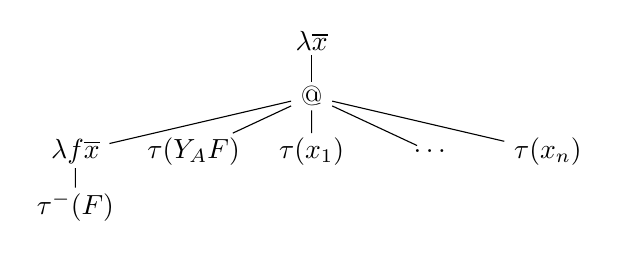
\begin{tikzpicture}[level distance=7mm,inner ysep=0.5mm,sibling distance=15mm,baseline=(r.base)]
\node (r)  {$\lambda \overline{x}$}
child {node{@}}
{
    child{node{$\lambda f \overline{x}$}
          child{node{$\tau^-(F)$}}
          }
    child{node{$\tau(Y_A F)$}}
    child{node{$\tau(x_1)$}}
    child{node{$\ldots$}}
    child{node{$\tau(x_n)$}}
};
\end{tikzpicture}
$$

for some fresh variables $\overline{x}:\overline{A}$ and where $\tau^-(F)$ denotes $\tau(F)$ with the root removed. This implies that $\tau(Y_A F) = \tau(F (Y_A F))$.


\begin{example}
Take $F \equiv \lambda f x. f x$. We have:
$$\elnf{Y F} \equiv \lambda x . \elnf{F} \elnf{Y F} \lambda.x \equiv \lambda x. (\lambda f x. f \lambda.x ) \elnf{Y F} \lambda.x$$ therefore its computation tree is the solution of the equation $\tau = \lambda x . (\lambda f x. f \lambda.x)~ \tau~(\lambda.x)$ in $\tau$.
\end{example}

We write $\travset_\tau(Y_A F)$ to denote the set of traversals of the computation tree $\tau(Y_A F)$.


\section*{A finite representation}

Since the subtree $\tau(Y_A F)$ in the second branch of the application node in $\tau(Y_A F)$ is the same tree as the main computation tree itself, we can identify them and remove the first one from the computation tree. This gives rise to a finite version $\widetilde\tau(Y_A F)$
of the computation tree:
$$\widetilde\tau(Y_A F) =
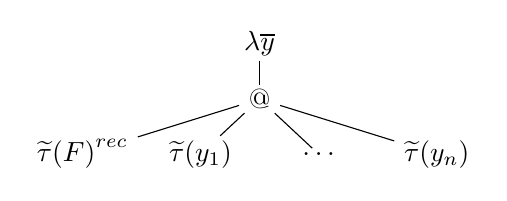
\begin{tikzpicture}[level distance=7mm,inner ysep=0.5mm,sibling distance=15mm,baseline=(r.base)]
\node (r)  {$\lambda \overline{y}$}
child {node{@}}
{
    child{node{${\widetilde\tau(F)}^{rec}$}}
    child{node{$\widetilde\tau(y_1)$}}
    child{node{$\ldots$}}
    child{node{$\widetilde\tau(y_n)$}}
};
\end{tikzpicture}
$$
where the exponent $rec$ means that the root of the subtree $\widetilde\tau(F)$ has a mark indicating that it is a special recursion lambda-node. The notion of traversal can be changed accordingly: Whenever a traversal meets a recursion variable $f$ in the subtree $\tau(F)$ then instead of jumping to the second child of the application node, it jumps to the root of the main tree. (Thus with this notion of traversal, the root can occur multiple times in the same traversal.) The definition of the mapping $\psi$ from nodes to moves remains consistent with this notion of computation tree, and the game-semantic correspondence still holds:
$$ \psi : \travset_{\widetilde\tau}( Y_A F )^{\filter \theroot} \stackrel{\cong}{\longrightarrow} \sem{Y_A F}$$
where $\travset_{\widetilde\tau}(M)^{\filter \theroot}$ denotes the set of reductions of traversals of the computation tree $\widetilde\tau(M)$.


\section*{An alternative finite representation}

In order to handle the $\ycomb$ combinators, we introduce a new kind of abstraction node. Such node is labelled $\lambda \overline{x}$ where each variable occurring in $\overline{x}$ is either a standard variable or a ``recursion variable''. Recursion variables are put into parenthesis in order to distinguish them from standard ones. The set $L$ of node labels is given by the grammar:
\begin{eqnarray*}
L &::=& \lambda\ V_{abs}^*\ |\ @\ |\ \mathcal{V} \\
V_{abs} &::=& \mathcal{V}\ |\ (\mathcal{V})
\end{eqnarray*}
for some countable set $\mathcal{V}$ of variables.


A term of the form $Y_A (\lambda f :A. M)$ where $M:A$ will be written  $\lambda (f) . M$. This notation also accounts for ground type recursion, for instance the \iawhile\ operator of Idealized Algol defined as $\iawhile\ C\ \iado\ I \equiv \ycomb ( \lambda f. \pcfcond\ C\ \iaskip\ (\iaseq\ I f))$ is rewritten as $\lambda (f) . \pcfcond\ C\ \iaskip\ (\iaseq\ I f)$.

To construct the computation tree of a PCF term, we first compute the $\eta$-long normal form as usual except for the $\ycomb$ combinator case which is treated as follows.
For each term $Y_A F$ where $F:A\rightarrow A$, let  $\elnf{F} = \lambda f \overline{x}. M$ where $f:A$ and $M:o$. The \emph{finite eta-normal form} of $Y_A F$ is defined to be
$\elnf{Y_A F} = \lambda (f) \overline{x} . M$.
The \defname{finite computation tree} is then obtained from the finite eta-normal form in the standard way:
$$\hat\tau(Y_A F) = 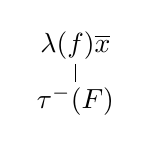
\begin{tikzpicture}[level distance=7mm,inner ysep=0.5mm,sibling distance=15mm,baseline=(r.base)]
\node (r)  {$\lambda (f) \overline{x}$}
child {node{$\tau^-(F)$}};
\end{tikzpicture}
$$


The definition of the  order of an abstraction node does not change:
it is the order of the term represented by the subtree rooted at
this node. In other word, the order of $\lambda \overline{x}$ is defined as the order of $\lambda \overline{y}$ where $\overline{y}$ is the sublist of $\overline{x}$  obtained by removing all the recursion variables in parenthesis.

The numbering of variables bound in a $\lambda$-node labelled $\lambda \overline{x}$ is as follows: The $i^{\sf th}$ standard variable in $\overline{x}$ is denoted by $i$ and the $i^{\sf th}$ recursion variable in $\overline{x}$ is denoted by $(i)$. The links in a justified sequence of nodes are labelled accordingly.

We can now define a notion of traversals adapted to this new kind of computation tree as follows. All the traversal rules are kept unmodified. The recursion variables in the $\lambda$-nodes are automatically ignored by the rules since such variables are numbered differently from standard variables. In particular, the (Var) rules only applies to non-recursion variables.
We add a new rule to handle recursion variable:
\begin{center}
\parbox{0.8\textwidth}{
\rulenamet{Var_{rec}}
If  \Pstr[0.6cm]{t' \cdot (n){n} \cdot (l){\lambda \overline{x}} \ldots (f-l,50:{(i)}){f_i}} is a traversal for some \emph{recursion} variable $f_i$ bound by $\lambda \overline{x}$ then so is \Pstr[0.6cm]{ t' \cdot (n){n} \cdot (l){\lambda \overline{x}}  \ldots (f-l,50:{(i)}){f_i} \cdot (letai-f){\lambda \overline{x}}}.
}
\end{center}

With the original definition of computation tree, the proof of
the Correspondence Theorem for \pcf\ was straightforward: It was done by a reduction
to the simply-typed lambda calculus case using the technique of approximants.
With the finite version of computation trees, it is not obvious to see which uncovering of moves gives rises to a correspondence with the set of traversals. However it is easy to show that the set of traversal reductions of the finite computation tree is equal to the set of traversal reductions of the standard computation tree. Therefore the Correspondence Theorem still holds.


\subsection*{Proof of soundness}

We now show that the finite representation $\hat\tau$ of a \pcf\ computation tree together with its set of traversals is equivalent to the original presentation.


We define a partial map $\alpha$ from the set of nodes of $\widetilde\tau(Y_A F)$ to the set of nodes of $\hat\tau(Y_A F)$ as follows. Each node labelled by a variable $x_i$ is mapped to the child of the root of the sub-tree $\tau(y_i)$ in $\widetilde\tau(Y_A F)$ labelled with $y_i$. Also, $\alpha$ maps each node hereditarily enabled by $x_i$ to the corresponding node hereditarily enabled by $y_i$ in $\widetilde\tau(Y_A F)$.

\begin{lemma}
$\alpha(\travset_{\hat\tau}(Y_A F)^{\filter \theroot}) =
\travset_{\widetilde\tau}(Y_A F)^{\filter \theroot}$.
\end{lemma}
\begin{proof}
We prove $\travset_{\widetilde\tau}(Y_A F)^{\filter \theroot} \subseteq
\alpha(\travset_{\hat\tau}(Y_A F)^{\filter \theroot})$ by induction on
the traversal rules for $\widetilde\tau$. The base case is trivial. For the
step case we consider the (Var) rule, the other cases being trivial.

Take the tree $\widetilde\tau$, when traversing the sub-tree $\tau^-(F)$, each time a variable node hereditarily justified by $\lambda (f) \overline{x}$ is encountered, the next step consists in taking a jump to a node in $\tau(y_i)$ hereditarily justified by the root of $\tau(y_i)$. Then the traversal of $\tau(y_i)$ continues until it reaches a variable node $z$ hereditarily justified by the root of $\tau(y_i)$ after which it jumps back to a node $\lambda \overline{\eta}$ in $\tau^-(F)$. $\lambda \overline{\eta}$ is the child of a previously visited node $p$ hereditarily justified by $\lambda (f) \overline{x}$ and from which a previous jump to $\tau(y_i)$ was taken:
$$ t = t_1 \cdot \underline{p} \cdot \lambda \overline{\nu} \cdot s \cdot z \cdot \underline{\lambda \overline{\eta}}$$
for some traversal $t_1$ of $\widetilde\tau$, sequence of nodes $s$ of even-length and where the nodes belonging to the sub-tree $\tau^-(F)$ are underlined.

By construction of $\tau(y_i)$, each node of $\tau(y_i)$ is either hereditarily justified by the root of $\tau(y_i)$
or by the root of $\widetilde\tau$. Consequently,
$$ t\filter r = (t_1\filter r) \cdot  (s \filter r) \ .$$

If $s = \epsilon$ then we conclude immediately using the induction hypothesis.
Suppose that $|s|\geq 2$ then $s = u\cdot \ldots \cdot v$ where $u$ the child of $\lambda \overline{\nu}$ and $v$ is the parent of $z$.
Necessarily, $u$ and $v$ are not hereditarily justified by the root of $\tau(y_i)$ and therefore are hereditarily justified by the root of $\widetilde\tau$. Hence:
$$ t\filter r = (t_1\filter r) \cdot  u \cdot v \ .$$

By the  induction hypothesis we have $t_1\filter r =
\alpha(t_1'\filter r)$ for some traversal $t_1'$  of $\hat\tau$.

The nodes $p$ and $\lambda \overline{\eta}$ belong
to the sub-tree $\tau^-(F)$ of $\widetilde\tau$. Let us write $p'$ and $\lambda \overline{\eta}'$ to denote the corresponding nodes in the sub-tree $\tau^-(F)$ of $\hat\tau$. We have $\alpha(p') = u$ and $\alpha(\lambda \overline{\eta}') = v$.

After the traversal $t_1'\filter r$ of $\hat\tau$, it is possible to
visit the node $p'$ using the same rule that has permitted to visit
$p$ in $\widetilde\tau$ after $t_1\filter r$. After this step, since $p'$ is
hereditarily justified by the root of $\hat\tau$, it is possible to
visit the child node $\lambda \overline{\eta}'$ of $p'$ using the
(InputVar) rule. Hence
$$(t_1'\filter r) \cdot p' \cdot \lambda \overline{\eta}' \in \travset(\hat\tau(Y_A F)) $$
and $\alpha((t_1'\filter r) \cdot p' \cdot \lambda \overline{\eta}')
= t\filter r$.

The proof of $\travset_{\widetilde\tau}(Y_A F)^{\filter \theroot} \supseteq
\alpha(\travset_{\hat\tau}(Y_A F)^{\filter \theroot})$ is similar.
\end{proof}

Although $\alpha$ is not injective (it maps two different nodes of $\hat\tau$ labelled by the same variable to the same node of $\widetilde\tau$), its node-wise extension to the set of reductions of traversals is injective.
The proof is by an easy induction on the traversal rules. Hence $\alpha$ defines an isomorphism from $\travset_{\widetilde\tau}(Y_A
F)^{\filter \theroot}$ to $\travset_{\hat\tau}(Y_A F)^{\filter
\theroot}$, and  consequently we have:
$$ \psi  \circ \alpha : \travset_{\hat\tau}( Y_A F)^{\filter \theroot} \stackrel{\cong}{\longrightarrow} \sem{Y_A F}$$
which shows that the finite representation $\hat\tau$ of the computation tree is sound in the sense that the game-semantics characterisation sill holds.

\end{document}
